
\section{Example: Storglaci{\"a}ren}\label{sec:storglaciaren} \index{Storglaci{\"a}ren}
\optsection{Storglaci{\"a}ren}

Storglaci{\"a}ren is a small valley glacier in northern Sweden (Figure~\ref{fig:storglaciaren}). The glacier is approximately 3.2\,km long and 1\,km wide, therefore much smaller than a single grid cell in a typical Greenland model. By the way ``Storglaci{\"a}ren'' means ``big glacier'' in Swedish. Most of the glacier is temperate, except for a thin cold near-surface layer in the ablation zone. Such a thermal structure is often-called a Scandinavian-type structure. Thanks to the nearby Tarfala research station it is one of the best investigated glaciers worldwide, and the wealth of data available makes it perfectly suitable for all kinds of modeling studies. In this tutorial we demonstrate how PISM can be used for valley glaciers, both in a 3-dimensional and a flow-line application. Additionally we show that PISM's conservation of energy scheme is able to simulate the glacier's polythermal structure.

\begin{figure}[ht]
  \centering
  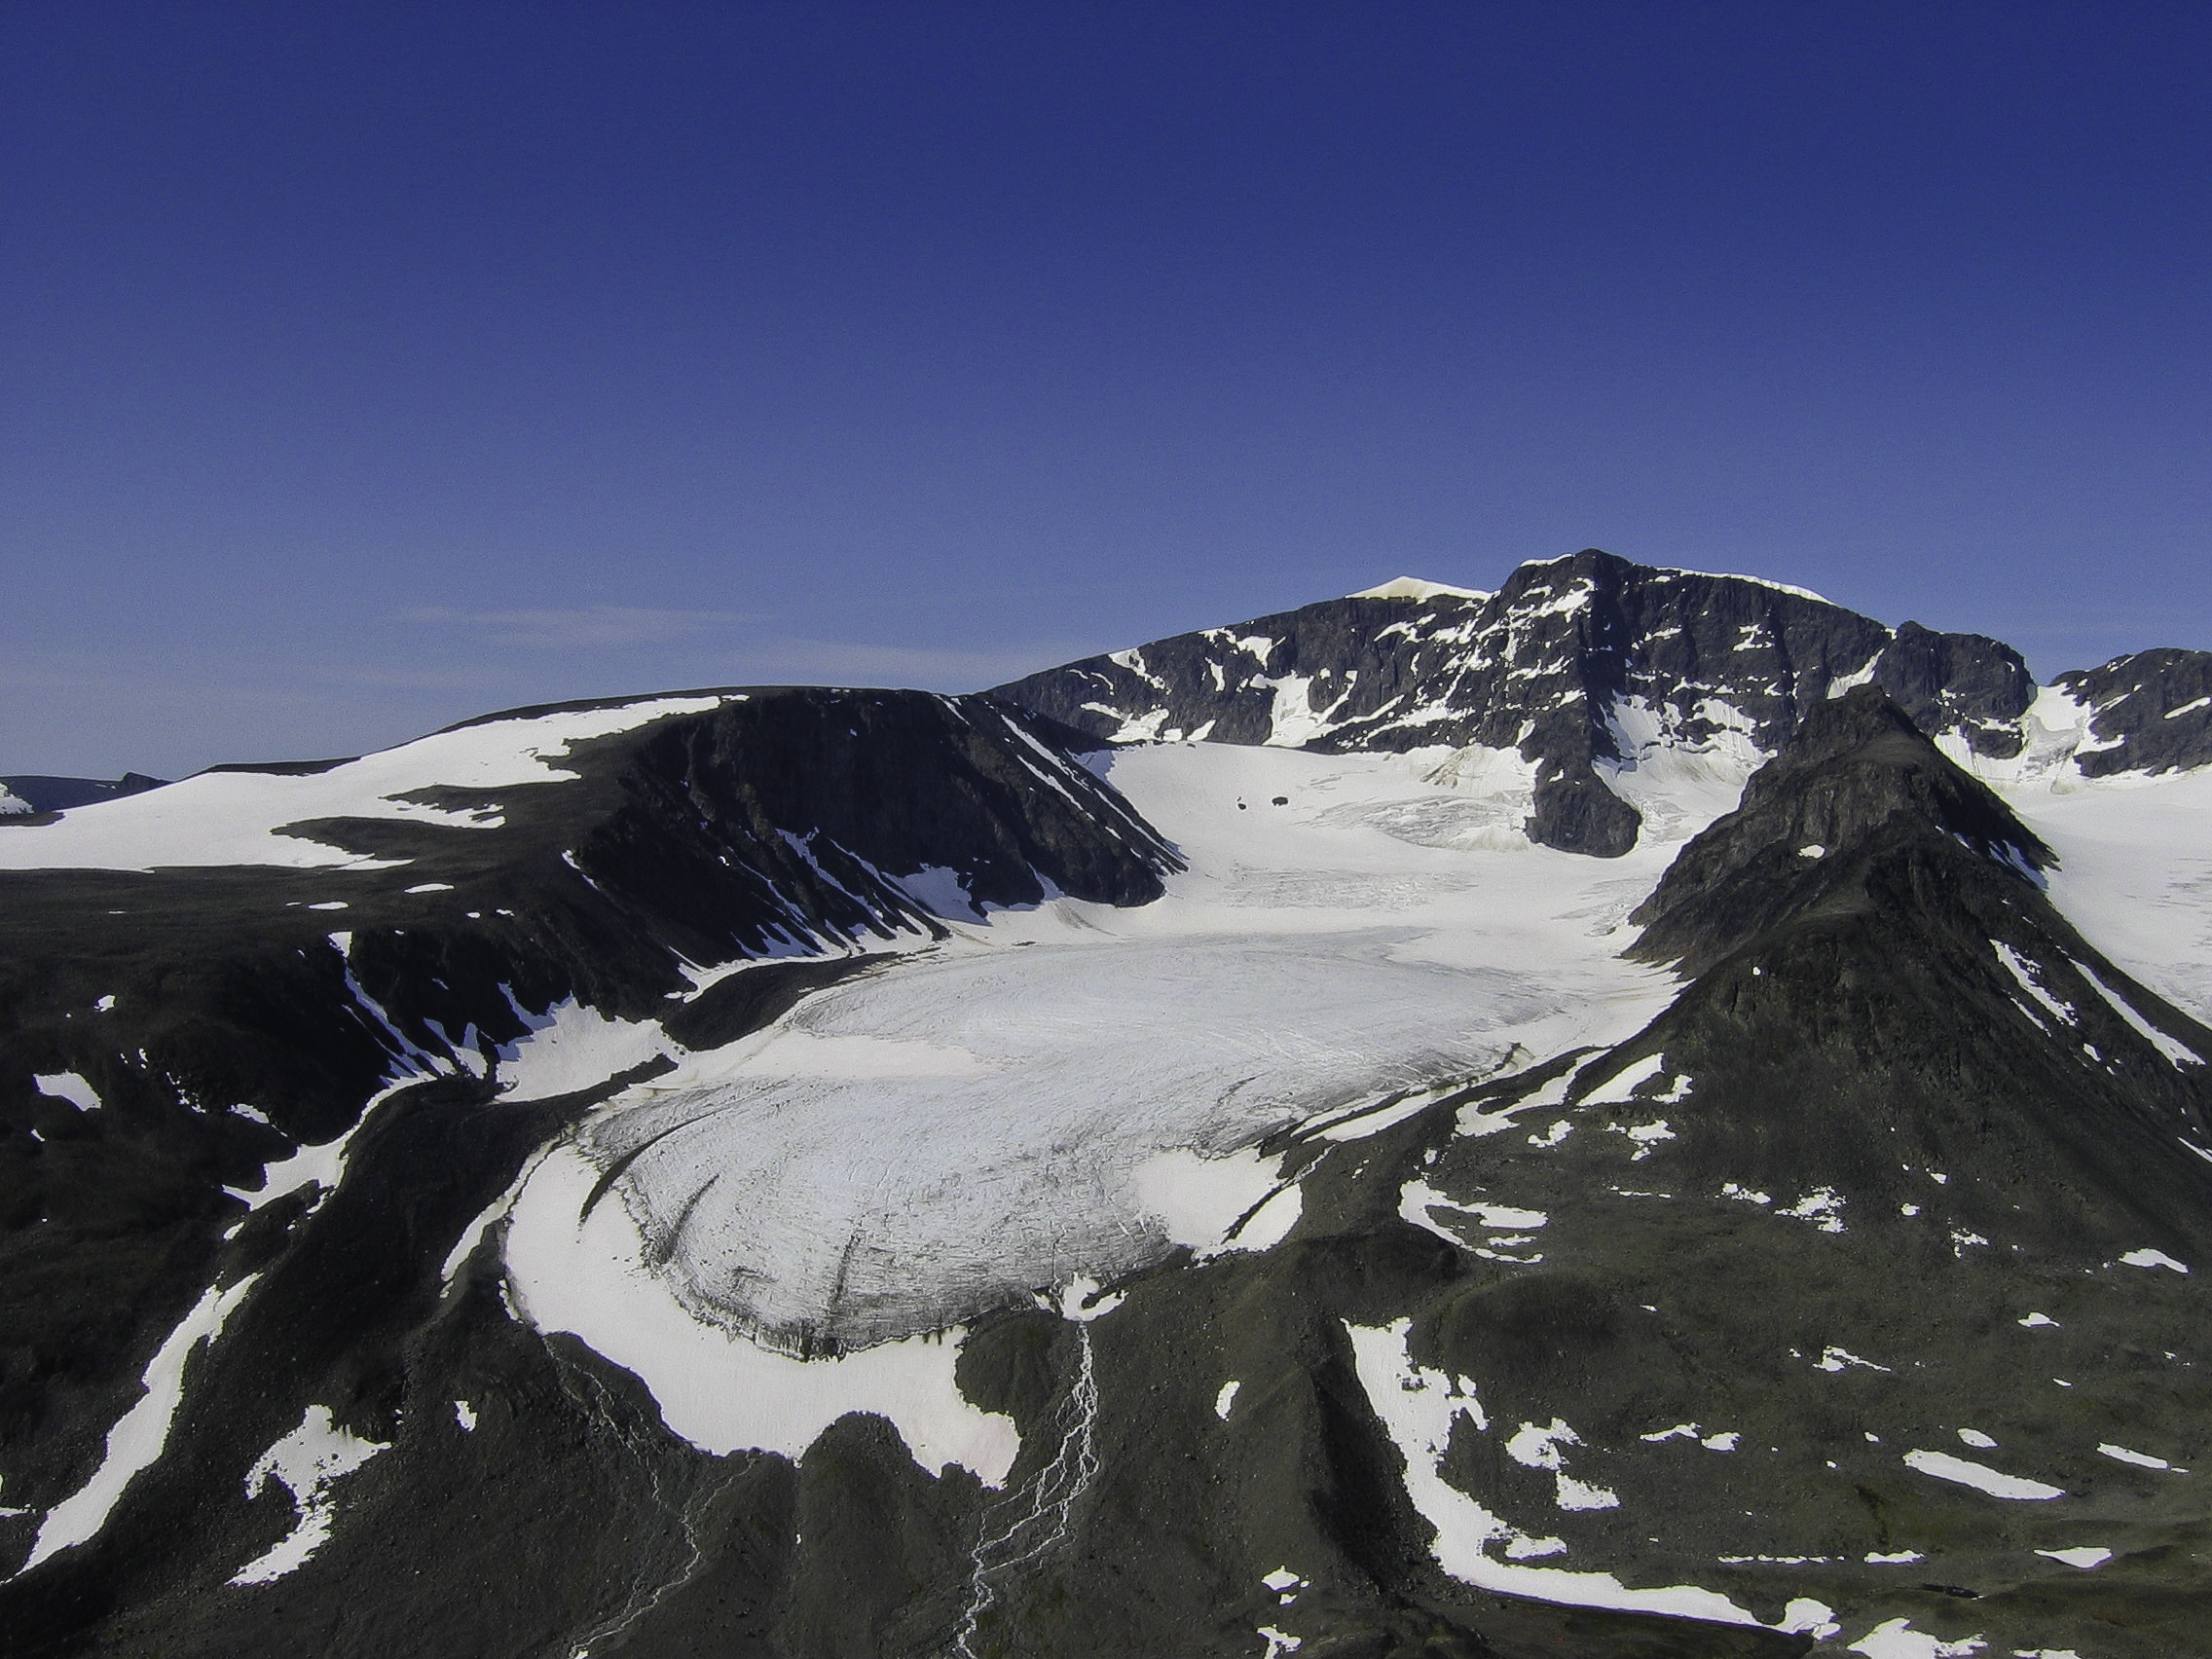
\includegraphics[width=3.in,keepaspectratio=true]{storglaciaren}\qquad
  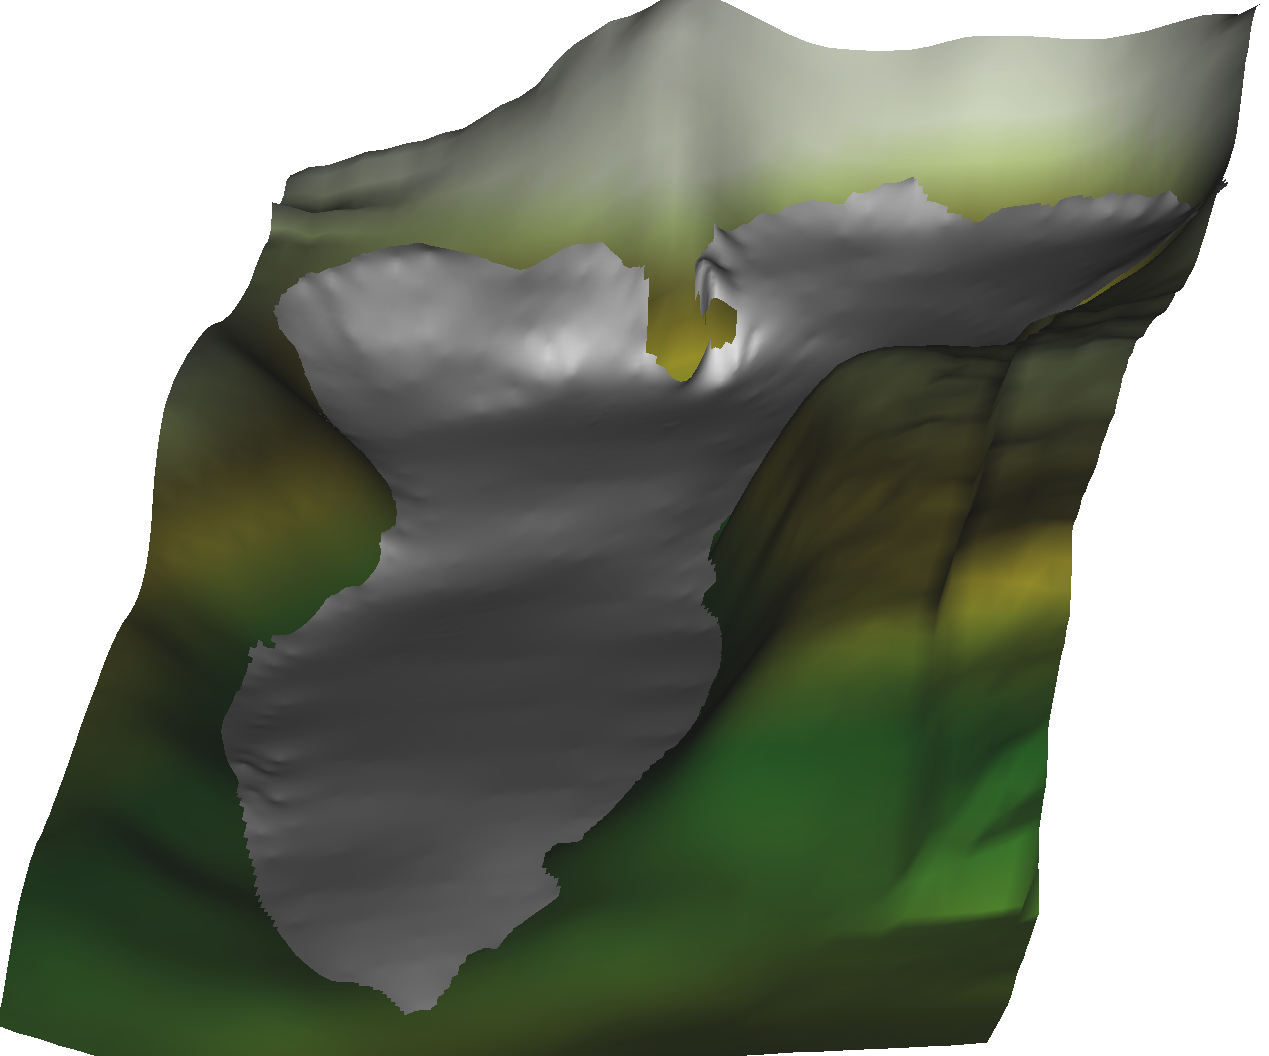
\includegraphics[width=2.75in,keepaspectratio=true]{storglaciaren-dem}
  \caption{Storglaci{\"a}ren, northern Sweden. Left: photo by R. Hock. Right: digital elevation model.}
  \label{fig:storglaciaren}
\end{figure}

The script \texttt{preprocess.sh} in \texttt{examples/storglaciaren} reads the digital elevation model from ASCII files and generates the necessary input files for both the 3-dimensional and the flow-line application. 

The mean annual air temperature $T_{\mathrm{MA}}=-6^{\circ}$C at the nearby Tarfala Research Stations serves as the boundary condition for the conservation of energy scheme below the firn line. Above it, where the ice is temperate, we choose 0$^{\circ}$C. 

\texttt{psg_flowline.sh} runs the flow-line application mode. The first two runs smooth the surface and create a more credible enthalpy field. In this example we want to infer the mass balance that has the present day geometry as a steady-state (for now, we ignore the fact that Storglaci{\"a}ren is probably not in a steady-state). As demonstrated in the third run, we can use PISM's mass balance modifier \texttt{-surface constant,forcing -force_to_thk psg_flowline_35m_steady.nc -force_to_thk_alpha 0.05}.

\begin{figure}[ht]
  \centering
  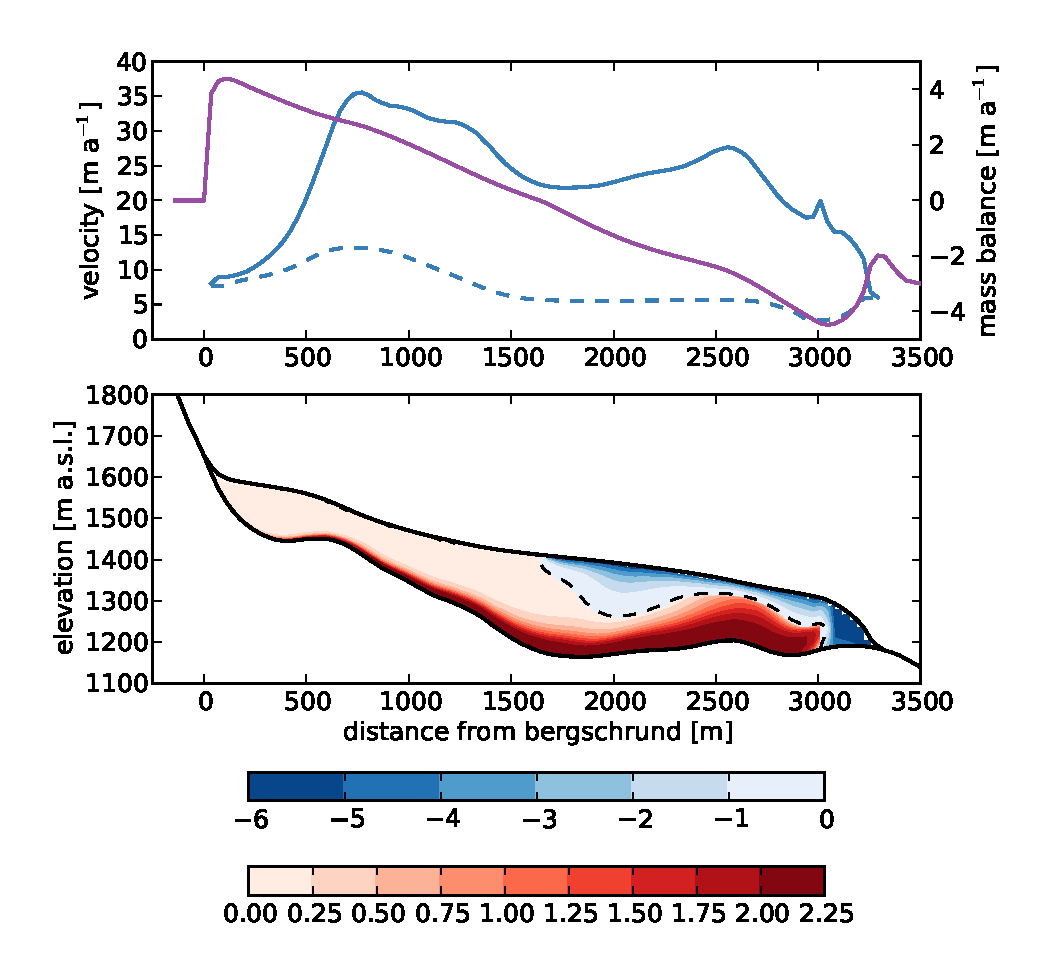
\includegraphics[width=5.in,keepaspectratio=true]{sg-flowline-ftt-result}
  \caption{Storglaci{\"a}ren, northern Sweden. Upper panel: horizontal surface velocity along flowline in meters per year. Lower panel: thermal structure. Red colors indicate liquid water content, blue colors are temperature in degrees Celsius}
  \label{fig:storglaciaren}
\end{figure}


The aim here model the steady-state configuration of the glacier given the following climatic conditions: \texttt{-surface elevation -acab -2.5,3.5,1100,1450,1660 -acab_limits -2.5,0}
